\documentclass[a4paper,12pt]{article}
\usepackage[utf8]{inputenc}
\usepackage[T1]{fontenc}
\usepackage[ngerman]{babel}

\usepackage{graphicx}
\usepackage[a4paper, left=3cm, right=2.5cm, top=3cm, bottom=3cm]{geometry}
\usepackage{setspace}
\onehalfspacing                % 1,5-facher Zeilenabstand
\setlength{\parindent}{0pt}    % Kein Einzug bei neuen Absätzen
\setlength{\parskip}{0.8em}    % Abstand zwischen Absätzen
\usepackage{parskip}

\usepackage{avant}
\renewcommand{\familydefault}{\sfdefault}

\usepackage{fancyhdr}
\setlength{\headheight}{14.5pt}
\pagestyle{fancy}
\fancyhf{}
\fancyhead[L]{\leftmark}
\fancyhead[R]{}
\fancyfoot[C]{\thepage}

\usepackage{titlesec}
\newcommand{\sectionbreak}{\clearpage}

\begin{document}
\sloppy

\begin{titlepage}
    \centering
    \begin{flushright}
        
\includegraphics[width=0.5\textwidth]{images/HFU-Logo.png}
    \end{flushright}
    
    \vspace{4cm}
    
    {\Large \textbf{Dokumentation}}\\[0.5cm]
    {\huge \textbf{Digitale Influencer}}\\[1.5cm]
    
    \textbf{Semesterprojekt Sommersemester 2025}
    
    \vfill
    
    \begin{flushleft}
    \textbf{Referent:} \\
    Herr Prof. Dr. Pascal Laube\\[2.5cm]
    
    \textbf{Autoren:} \\
    Marvin Jonas Kern \\
    Kevin Maisler \\
    Julia Maria Riebel \\
    Bünyamin Sener \\
    \end{flushleft}
    
    \vfill
    \begin{center}
        {\large \today}
    \end{center}
\end{titlepage}

\renewcommand*\contentsname{Inhaltsverzeichnis}
\tableofcontents
\newpage

\section{Einleitung}
Im Sommersemester 2025 wurde im Rahmen der Studiengänge \textit{Angewandte Informatik} und \textit{IT-Produktmanagement} an der Hochschule Furtwangen ein interdisziplinäres Projekt mit dem Titel \textit{„Digitale Influencer – Aufbau einer virtuellen Social-Media-Präsenz“} durchgeführt. Unter der Betreuung von Prof. Dr. Pascal Laube arbeitete ein vierköpfiges Studierendenteam daran, innerhalb eines Semesters eine vollständig digitale Influencer-Persona zu konzipieren, technisch umzusetzen und auf relevanten sozialen Netzwerken sichtbar zu machen und strategisch zu etablieren. \\\\
Ziel des Projekts war es, mithilfe moderner KI-Tools eine virtuelle Influencer-Persönlichkeit zu erschaffen, die durch automatisiert erstellte Foto- und Videoinhalte eine möglichst hohe Reichweite sowie ein nachhaltiges Followerwachstum generieren kann. Im Mittelpunkt standen dabei der Aufbau einer eigenständigen digitalen Identität, die KI-gestützte Content-Erstellung (Text, Bild, Video) sowie die algorithmisch optimierte Ausspielung und Interaktion auf Plattformen wie Instagram und TikTok.\\\\
Neben der technischen Umsetzung umfasste das Projekt auch kreative, analytische und organisatorische Aufgaben: von der Recherche aktueller Social-Media-Trends über das Prompt-Engineering für die Contentgenerierung bis hin zur kontinuierlichen Auswertung von Engagement-Daten zur Strategieoptimierung. Auch der Umgang mit APIs (Meta Graph API), die Automatisierung täglicher Abläufe (via GitHub Actions) sowie der Einsatz datengetriebener Analyseverfahren (z.B. zur Follower-Strukturanalyse) waren zentrale Bestandteile der Arbeit.\\\\
Die besondere Herausforderung bestand darin, technologische Innovation mit kreativem Storytelling zu verbinden – eine  Aufgabe, die ein hohes Maß an Teamarbeit, Eigenverantwortung, Experimentierfreude und digitaler Affinität erforderte. Darüber hinaus mussten auch rechtliche Rahmenbedingungen berücksichtigt werden, insbesondere im Hinblick auf Urheberrechte, Persönlichkeitsrechte und die Nutzung von KI-generierten Inhalten auf öffentlichen Plattformen. Durch die Kombination aus KI-gestützter Automatisierung, datengetriebener Strategie und Kreativität wurde ein zukunftsweisendes Modell für virtuelle Influencer-Projekte im Hochschulkontext entwickelt.


\newpage

\section{Vorbereitungen}
Bevor wir mit der eigentlichen Umsetzung starten konnten, mussten ein paar grundlegende Fragen geklärt werden: Was ist rechtlich erlaubt? Welche Zielgruppe wollen wir überhaupt ansprechen? Und mit welchen Tools können wir das Ganze technisch realisieren? Dieses Kapitel fasst die wichtigsten Überlegungen und Recherchen zusammen, die wir zu Beginn des Projekts angestellt haben.

\subsection{Rechtliche Ausgangslage}

Die Entwicklung und Veröffentlichung eines digitalen Influencers bringt verschiedene rechtliche Fragestellungen mit sich – insbesondere im Hinblick auf Bildgenerierung, automatisierte Interaktion und Social-Media-Plattformrichtlinien. In diesem Abschnitt werden die wichtigsten Rahmenbedingungen für Deutschland sowie relevante Vorgaben der Plattform Instagram erläutert.

\subsubsection*{Bildgenerierung und Urheberrecht}

KI-gestützte Bildgenerierung durch Tools wie Stable Diffusion oder DALL·E wirft in Deutschland urheberrechtliche Fragen auf. Generell gilt: Solange die erstellten Inhalte ohne wesentliche kreative Eigenleistung entstehen (z.\,B. durch einfache Prompts), sind sie urheberrechtlich meist nicht geschützt. 

Beim Training solcher Modelle dürfen – unter Berücksichtigung der EU-Richtlinie zum Text-und-Data-Mining – auch urheberrechtlich geschützte Bilder verwendet werden, sofern die Nutzung nicht kommerziell erfolgt oder Rechteinhaber dem nicht ausdrücklich widersprochen haben (z.\,B. über \texttt{robots.txt} oder \texttt{ai.txt}). Für die praktische Umsetzung bedeutet das: Bei rein akademischem Einsatz ist die Nutzung von öffentlich verfügbaren Modellen in der Regel unproblematisch.

\subsubsection*{Plattformrichtlinien und Digital Services Act (DSA)}

Mit dem Inkrafttreten des EU Digital Services Act (DSA) wurden neue Regeln für den Umgang mit Inhalten auf Plattformen wie Instagram eingeführt. Auch wenn sich viele Bestimmungen direkt an die Betreiber der Plattformen richten, ergeben sich daraus indirekt auch Pflichten für Content-Ersteller:innen – insbesondere dann, wenn KI-generierte Inhalte oder automatisierte Prozesse zum Einsatz kommen.

Ziel des DSA ist es, für mehr Transparenz, Fairness und Sicherheit im digitalen Raum zu sorgen.
Auch wenn unser Projekt keine kommerziellen oder sicherheitsrelevanten Inhalte verbreitet, ist es wichtig, bei der Planung und Veröffentlichung transparenter, KI-generierter Inhalte auf die gestiegene gesellschaftliche Sensibilität gegenüber „nicht-menschlichen Akteuren“ zu achten. Der DSA fordert genau diese Offenheit und Nachvollziehbarkeit.

\subsubsection*{Automatisierte Interaktion und DSGVO}

Die automatisierte Interaktion über Instagram (z.\,B. Antworten auf Nachrichten) unterliegt strengen Vorgaben. Laut den offiziellen \textbf{Meta-Richtlinien} ist Automatisierung ausschließlich über die \textit{Instagram Graph API} erlaubt und nur dann zulässig, wenn:

\begin{itemize}
    \item Nutzer:innen die Konversation initiieren (24-Stunden-Regel),
    \item ein verifizierter Business-Account verwendet wird
    \item eine deutliche Information darüber erfolgt, dass es sich um automatisierte Kommunikation handelt.
\end{itemize}

Unzulässig sind dagegen:
\begin{itemize}
    \item unaufgeforderte Nachrichtenversendungen,
    \item das Umgehen der API über Scraper oder inoffizielle Tools
    \item die Nutzung privater oder Creator-Accounts für Automatisierung.
\end{itemize}

Darüber hinaus gelten die Vorgaben der DSGVO: Vor der Verarbeitung personenbezogener Daten (z.\,B. bei Chatbots oder Analytics) ist eine informierte Einwilligung erforderlich. Nutzer:innen müssen über Art, Umfang und Zweck der Datenverarbeitung aufgeklärt werden. Außerdem müssen Daten sicher gespeichert, auf Wunsch gelöscht und vor unbefugtem Zugriff geschützt werden.

\subsubsection*{Zusammenfassung}

Für unser Projekt bedeutet das konkret:

\begin{itemize}
    \item KI-generierte Inhalte dürfen genutzt werden, solange keine Rechte Dritter verletzt werden.
    \item Interaktionen müssen transparent als automatisiert gekennzeichnet sein.
    \item Die Kommunikation erfolgt ausschließlich über von Meta freigegebene Schnittstellen.
    \item Die datenschutzrechtlichen Anforderungen der DSGVO müssen eingehalten werden.
\end{itemize}

Die Einhaltung dieser Rahmenbedingungen war eine wichtige Grundlage für die technische und konzeptionelle Umsetzung des Projekts.


\subsection{Marktanalyse}

Die Entwicklung eines digitalen Influencers erfordert ein fundiertes Verständnis der aktuellen Markt- und Zielgruppenlage. In diesem Zusammenhang wurden sowohl bestehende Trends im Bereich virtueller Persönlichkeiten als auch konkrete Plattformdaten analysiert, um die strategische Ausrichtung des Projekts zu begründen.

\subsubsection*{Aktuelle Trends und Relevanz}

Virtuelle Influencer haben in den letzten Jahren stark an Bedeutung gewonnen. Digitale Persönlichkeiten wie Lil Miquela, Lu do Magalu oder Aitana Lopez erreichen auf Social Media beachtliche Reichweiten – ganz ohne physische Existenz. Gleichzeitig erleben Themen wie Persönlichkeitsentwicklung, Coaching und Mental Health einen regelrechten Boom.

Besonders auffällig ist, dass die Akzeptanz gegenüber KI-generierten Inhalten bei der Generation Z und den Millennials kontinuierlich steigt. Diese Zielgruppen sind offen für neue Formate, digitale Experimente und alternative Identifikationsfiguren. Genau das sind ideale Voraussetzungen für unser Konzept: ein KI-gestützter, inspirierender und beratender Influencer mit einem positiven, motivierenden Charakter.

\subsubsection*{Wettbewerbsanalyse}

Eine gezielte Wettbewerbsanalyse zeigte, dass der Markt für virtuelle Influencer:innen mit mentorartigem Fokus bisher kaum besetzt ist. Während viele menschliche Creator wie Ali Abdaal oder Mel Robbins Inhalte mit Coaching-Charakter anbieten, gibt es aktuell nur sehr wenige digitale Persönlichkeiten mit vergleichbarem thematischem Schwerpunkt. Diese Nische bietet somit eine klare Möglichkeit zur Differenzierung und Positionierung.

\subsubsection*{Zielgruppenanalyse}

Basierend auf unserer Recherche und den Plattformdaten haben wir folgende Zielgruppe definiert:

\begin{itemize}
    \item \textbf{Alter:} 16–35 Jahre
    \item \textbf{Geschlecht:} alle
    \item \textbf{Bildung:} Schüler:innen, Studierende, Berufseinsteiger:innen
    \item \textbf{Bedürfnisse:} Motivation, Struktur, Inspiration, Karriereorientierung
    \item \textbf{Werte:} Offenheit, Selbstreflexion, digitale Affinität
    \item \textbf{Pain Points:} Überforderung, Prokrastination, mangelnde Orientierung
    \item \textbf{Verhalten:} tägliche Nutzung sozialer Medien, bevorzugt kurze motivierende Inhalte (z.\,B. Reels oder Zitat-Posts), aktive Beteiligung durch Likes, Kommentare und Story-Interaktionen
\end{itemize}

\subsubsection*{Plattformwahl}

Die Wahl der Plattform fiel auf Instagram, da sie in mehrfacher Hinsicht optimal zu unserer Zielgruppe passt. Mit über 30 Millionen aktiven Nutzer:innen allein in Deutschland – der Großteil davon zwischen 18 und 34 Jahren – bietet Instagram eine hervorragende Ausgangsbasis für Reichweite und Community-Aufbau.

Vorteile von Instagram im Überblick:

\begin{itemize}
    \item Visuelle Ausrichtung: ideal für ästhetisch gestalteten Content
    \item Vielfältige Formate: Reels, Karussell-Posts, Storys, Highlights
    \item Hohe Interaktionsmöglichkeiten: z.\,B. über Likes, Kommentare, Umfragen, DMs
    \item Algorithmische Sichtbarkeit: gerade für neue Accounts mit relevantem Content
\end{itemize}

Zudem lassen sich durch einheitliches Design (Farben, Schrift, visuelle Tonalität), gezielte Hashtag-Strategien und optimale Posting-Zeiten starke Wiedererkennungswerte schaffen. Besonders hohe Aktivitätsraten konnten wir für Posts am Wochenende sowie in den späten Nachmittags- und Abendstunden (16–21 Uhr) feststellen.

\subsubsection*{Weitere Plattformen}

Auch wenn Instagram im Mittelpunkt steht, wurden zu Beginn des Projekts weitere Plattformen wie TikTok, YouTube und LinkedIn in die Analyse einbezogen:

\begin{itemize}
    \item \textbf{TikTok:} Kurzform-Videos mit motivierendem Charakter
    \item \textbf{YouTube:} Potenzial für längere Tutorials oder Deep-Dive-Videos
    \item \textbf{LinkedIn:} Optionale Ergänzung für karrierebezogene Inhalte im professionellen Umfeld
\end{itemize}

Für den Projektzeitraum wurde Instagram als Hauptplattform ausgewählt – unter anderem aufgrund der einfacheren API-Anbindung, der Formatvielfalt und der direkten Zielgruppenansprache. Andere Plattformen könnten im Rahmen einer späteren Skalierung in Betracht gezogen werden.


\subsection{Toolrecherche}

Um die Anforderungen unseres Projekts – insbesondere die vollautomatisierte Generierung realistischer Inhalte für eine digitale Influencer-Persona – bestmöglich umzusetzen, haben wir verschiedene Softwarelösungen recherchiert und bewertet. Dabei lag der Fokus auf Tools, die sich zuverlässig automatisieren lassen, kostenfrei oder zumindest günstig nutzbar sind und konsistente Ergebnisse liefern – sowohl im Bild-, Video- als auch im Textbereich.

\textbf{Unsere Hauptkriterien bei der Toolauswahl:}
\begin{itemize}
    \item Realistische Bildqualität
    \item Automatisierbarkeit über eine API (z.\,B. mit Python)
    \item Kostenfreiheit oder kostengünstige Nutzung
    \item Open-Source-Verfügbarkeit
    \item Konsistente Bildausgabe für ein gleichbleibendes Gesicht
\end{itemize}

\subsubsection{Bildgenerierung}

\paragraph{ChatGPT (mit DALL·E)}
Die Plus-Version von ChatGPT enthält das KI-Bildgenerierungstool DALL·E, das qualitativ hochwertige Bilder erzeugt und auch Funktionen wie Inpainting unterstützt. Die größte Einschränkung: Es gibt aktuell keine öffentlich nutzbare API zur Bildgenerierung. Die Nutzung erfolgt ausschließlich über die Weboberfläche, was eine Automatisierung für unser Projekt ausschließt. Zudem ist eine kostenpflichtige Lizenz erforderlich.

\paragraph{Stability AI (Stable Diffusion API)}
Stability AI bietet mit Stable Diffusion eine leistungsstarke Bildgenerierungs-API, die prinzipiell eine vollständige Integration in eigene Workflows ermöglicht. Die Nutzung erfolgt jedoch über ein Credit-basiertes System, sodass bei regelmäßigem Einsatz relevante Kosten entstehen können. Für große Volumen oder tägliche Bildproduktion ist das wirtschaftlich nicht ideal.

\paragraph{Hugging Face}
Hugging Face stellt zahlreiche Open-Source-Modelle zur Verfügung, darunter Stable Diffusion, DreamBooth oder ControlNet. Viele dieser Modelle lassen sich über eine API automatisieren und auch kostenfrei testen. Je nach Nutzungslast kann es jedoch zu Einschränkungen bei Rechenzeit und Antwortgeschwindigkeit kommen.

\paragraph{Fooocus}
Fooocus ist eine besonders anwenderfreundliche Open-Source-Variante zur Bildgenerierung auf Basis von Stable Diffusion. Das Tool vereinfacht die Konfiguration komplexer Modelle und lässt sich lokal installieren. Dadurch entstehen keine laufenden Kosten, und es ist keine Cloud-Anbindung erforderlich. Unterstützt werden moderne Features wie Inpainting, Upscaling und ControlNet.

\subsubsection{Textgenerierung}

\paragraph{Ollama}
Ollama ist eine Laufzeitumgebung zur lokalen Ausführung von Large Language Models (LLMs) wie LLaMA 3, Mistral oder Zephyr. Sie eignet sich besonders für lokale Automatisierung ohne Cloud-Anbindung. Die Nutzung erfolgt über eine einfache CLI-Schnittstelle, was den Einsatz in Python-Skripten erleichtert.

\paragraph{OpenAI GPT (Playground / API)}
OpenAIs GPT-Modelle bieten hervorragende Textqualität und viele Einsatzmöglichkeiten. Allerdings ist die Nutzung kostenpflichtig, erfordert eine API-Registrierung und ist nicht datenschutzkonform, wenn persönliche Daten verarbeitet werden. Eine lokale Ausführung ist nicht möglich. Zudem lässt sich der Webzugang (Playground) nicht automatisieren.

\paragraph{Hugging Face Transformers}
Auch im Textbereich bietet Hugging Face viele vortrainierte Sprachmodelle. Diese lassen sich entweder lokal oder über die Cloud betreiben. Die Plattform ist offen und gut dokumentiert. Technisch erfordert die Einrichtung jedoch mehr Aufwand, und viele Modelle sind leistungsmäßig schwächer als ihre Konkurrenten.

\paragraph{Google Gemini (ehemals Bard)}
Gemini ist Googles KI-Textgenerator, der über eine benutzerfreundliche Weboberfläche genutzt werden kann. Die Ergebnisse sind sprachlich ansprechend, doch es gibt keine API-Zugänglichkeit. Für automatisierte Workflows ist das Tool daher ungeeignet.

\subsubsection{Videogenerierung}

\paragraph{HeyGen AI}
Heygen ist ein cloudbasiertes KI-Tool zur automatisierten Generierung von Videoinhalten mit fotorealistischen Avataren. Nutzer*innen können mithilfe von Text-zu-Video-Technologie realistische Sprecher-Videos erstellen, in denen digitale Charaktere (Avatare) auf Basis eingegebener Texte synthetisch sprechen. Besonders für Marketing, Erklärvideos oder Social-Media-Content eignet sich das Tool aufgrund seiner schnellen Ergebnisse und breiten Vorlagenbibliothek.

Heygen bietet eine intuitive Benutzeroberfläche und unterstützt Multisprachen-Synthese mit natürlicher Sprachmelodie. Eine automatisierte Ansteuerung ist derzeit nicht direkt über eine öffentliche API möglich; der Fokus liegt auf einer webbasierten Nutzung. Für einfache Anwendungen reicht ein kostenfreier Account mit limitierten Videominuten. Weiterführende Funktionen, wie längere Videos oder eine höhere Avataranzahl, sind nur in den kostenpflichtigen Versionen verfügbar.

\paragraph{Pika}
Pika ist ein KI-gestütztes Text-zu-Video-Tool, das sich auf die kreative Generierung kurzer, animierter Videos spezialisiert hat. Die Plattform erlaubt es, aus einem Textprompt oder Bildvorgaben dynamische Clips mit Bewegungen, Kameraeffekten und stilisierten Elementen zu erzeugen. Pika richtet sich primär an kreative Content-Creatorinnen und Designerinnen, die schnell visuelle Konzepte umsetzen möchten.

Die Nutzung erfolgt über eine grafische Weboberfläche. Eine automatisierte Ansteuerung über API ist aktuell nicht öffentlich dokumentiert, wobei der Anbieter regelmäßig neue Funktionen in der Beta-Phase testet. Die generierten Videos sind stark stilisiert und eignen sich insbesondere für experimentellen, visuellen Social-Media-Content. Pika kann in der Basisversion kostenlos genutzt werden, es bestehen jedoch maßgebliche Einschränkungen hinsichtlich Renderzeit, Auflösung und Anzahl der Videos.

\clearpage

\section{Auswahl der Technologien}
Die technische Umsetzung unseres Projekts basierte auf einem bewusst schlank gehaltenen Technologie-Stack, der einfache Automatisierung und hohe Flexibilität vereint. In diesem Kapitel werden die eingesetzten Kerntechnologien beschrieben – inklusive ihrer konkreten Rolle im Projekt, der Vorteile gegenüber Alternativen sowie der Gründe für ihre Auswahl.

\subsection{Python}

Python wurde im Projekt als zentrale Programmiersprache eingesetzt und bildete die technische Grundlage für nahezu alle automatisierten Prozesse. Die Sprache eignet sich besonders gut für die Kombination aus künstlicher Intelligenz, Web-APIs und Automatisierungslogik – drei Kernbereiche, die das Projekt vereinte. Die klare Syntax, die starke Community und die riesige Auswahl an verfügbaren Bibliotheken machen Python zu einem bevorzugten Werkzeug für schnelle Entwicklung und zuverlässige Integration.

Im Projektkontext wurde Python genutzt, um Bild- und Textgenerierungsprozesse zu steuern, lokale KI-Modelle anzusprechen (z.\,B. über die Kommandozeile mit Ollama), Bilddateien zu verwalten, sowie automatisierte Inhalte an Instagram zu übermitteln. Dafür kamen unter anderem Bibliotheken wie \texttt{subprocess} (zur Systemansteuerung), \texttt{os} (Dateioperationen), \texttt{requests} (API-Kommunikation), \texttt{json} (Datenstrukturierung) und \texttt{schedule} (Task-Planung) zum Einsatz.

Ein entscheidender Vorteil lag in der nahtlosen Integration mit GitHub Actions, wodurch sich Python-Skripte zeit- oder ereignisbasiert auf einem Server ausführen ließen – ganz ohne manuelles Eingreifen. So konnten beispielsweise neue Inhalte vollautomatisch generiert und veröffentlicht werden, sobald ein geplanter Posting-Zeitpunkt erreicht war.

Auch komplexere Prozesse wie die Auswahl passender Hashtags, das Einbinden von Variablen in Texttemplates oder der Umgang mit unterschiedlichen Inhaltsformaten ließen sich in Python übersichtlich und modular abbilden. Python ermöglichte es dem Team, technische Flexibilität mit klarer Wartbarkeit zu verbinden – ein wesentlicher Erfolgsfaktor im Hinblick auf die Skalierbarkeit und Wiederverwendbarkeit des Projektcodes.

\subsection{Github}

GitHub diente im Projekt nicht nur als zentrales Versionsverwaltungssystem, sondern spielte auch eine tragende Rolle in der automatisierten Ausführung der technischen Abläufe. Über die Plattform wurde der gesamte Quellcode entwickelt, dokumentiert und versioniert. GitHub ermöglichte es dem Team, effizient verteilt zu arbeiten, Änderungen nachzuvollziehen und reproduzierbare Ergebnisse zu sichern.

Besonders zentral war der Einsatz von GitHub Actions. Damit konnten Workflows definiert werden, die auf bestimmte Ereignisse reagieren – etwa das Hinzufügen neuer Bilddateien, geplante Zeitpunkte oder manuelle Trigger. Die automatisierte Generierung und Veröffentlichung von Social-Media-Inhalten basierte auf diesen Workflows. So wurde unter anderem bei jedem neuen Bild automatisch ein Python-Skript ausgeführt, das sowohl Text generierte (via Ollama) als auch Bild und Beschreibung über die Meta Graph API an Instagram übermittelte.

Für den sicheren Umgang mit sensiblen Informationen wie API-Zugängen oder Tokens wurden die GitHub Secrets genutzt. Sie ermöglichten es, vertrauliche Daten wie Zugriffstoken für die Meta-Plattform oder interne Variablen sicher im Repository zu hinterlegen, ohne dass diese im Quellcode sichtbar waren. Die Secrets wurden automatisch zur Laufzeit der Actions in das jeweilige Skript eingebunden und konnten so ohne manuelle Eingabe sicher verwendet werden.

Ein weiterer Vorteil von GitHub Actions war die einfache Wartbarkeit und Erweiterbarkeit: neue Automatisierungsschritte konnten modular ergänzt werden, etwa für Statusanzeigen, Log-Dateien oder Validierungen. Die Kombination aus Versionskontrolle, Automatisierung und sicherem Geheimnismanagement machte GitHub zu einem zentralen Baustein für die technische Struktur und Effizienz des Projekts.

\subsection{Ollama}

Ollama wurde im Projekt als Laufzeitumgebung für lokal ausgeführte Large Language Models (LLMs) eingesetzt und bildete das Kernstück der automatisierten Textgenerierung. Das Tool ermöglicht es, moderne Sprachmodelle wie LLaMA~3, Mistral oder Zephyr direkt auf dem eigenen System zu betreiben – ohne Abhängigkeit von externen Cloud-Diensten. Diese Eigenschaft war ein zentraler Entscheidungsfaktor im Hinblick auf Datenschutz, Automatisierbarkeit und Unabhängigkeit.

Durch die schlanke Kommandozeilen-Schnittstelle ließ sich Ollama problemlos in Python-Skripte einbinden und konnte so im Rahmen automatisierter Workflows verwendet werden. Das Tool eignete sich besonders für die Generierung von Social-Media-Captions, Hashtag-Blöcken und Beschreibungstexten, da es auf vorgefertigte Prompts reagieren und konsistente Ergebnisse liefern konnte. Die generierten Texte wurden anschließend automatisch weiterverarbeitet und in die Post-Logik integriert.

Ein zusätzlicher Vorteil lag in der lokalen Kontrolle über das Modellverhalten und den Prompt-Flow: Experimentelle Anpassungen konnten sofort umgesetzt werden, ohne dass externe Abhängigkeiten berücksichtigt werden mussten. Zudem war die Nutzung von Ollama vollständig kostenlos und auch auf leistungsschwächerer Hardware praktikabel.

Im Gesamtprojekt spielte Ollama damit eine Schlüsselrolle in der textuellen Content-Produktion – effizient, lokal ausführbar und vollständig automatisierbar.

\subsection{Fooocus}

Nach der Analyse verschiedener KI-gestützter Bildgenerierungstools fiel die finale Wahl auf Fooocus. Das Open-Source-Tool erfüllte sämtliche Anforderungen unseres Projektes in Bezug auf Bildqualität, Konsistenz, Kostenfreiheit, Automatisierbarkeit und lokale Nutzbarkeit.

Fooocus basiert auf dem Modell Stable Diffusion und verfolgt einen benutzerfreundlichen Ansatz. Statt komplexer technischer Einstellungen konzentriert sich die Nutzung auf die Eingabe eines Prompts, also einer textuellen Beschreibung des gewünschten Bildinhalts. Alle weiteren Parameter wie Stil, Sampler, Bildgröße oder Upscaling werden im Hintergrund automatisch optimiert. Dies erleichtert nicht nur den Einstieg, sondern ermöglicht auch eine schnelle und konsistente Generierung hochwertiger Bilder. \\\\
Ein besonderer Vorteil von Fooocus im Kontext unseres Projekts ist die Fähigkeit, stilistisch einheitliche und visuell konsistente Bildserien zu erzeugen. Für die digitale Persona war es entscheidend, dass das Gesicht über viele Beiträge hinweg wiedererkennbar bleibt. Fooocus unterstützt hierfür moderne Technologien wie ControlNet, Inpainting und VAE-Optimierungen, mit denen sich gezielt Details im Bild verändern lassen, ohne das Gesamtbild zu verfälschen.

Durch die Open-Source-Lizenz bietet Fooocus volle Kontrolle über die Software sowie eine lokale Ausführbarkeit ohne laufende Kosten. Dies ermöglichte eine flexible Integration in bestehende Workflows und bildete eine solide Grundlage für die spätere Automatisierung des Bildgenerierungsprozesses. 

Fooocus kann sowohl über eine grafische Weboberfläche lokal im Browser bedient werden als auch über eine lokal gehostete API-Schnittstelle angesprochen werden. Für die finale Umsetzung der automatisierten Bildgenerierung wurde die API-Variante eingesetzt, da sie eine direkte Ansteuerung über Python ermöglichte und sich nahtlos in den bestehenden Automatisierungsworkflow integrieren ließ.


\subsection{Meta Graph API}

Die Meta Graph API wurde im Projekt verwendet, um Inhalte automatisiert auf Instagram zu veröffentlichen. Sie stellt die offizielle Schnittstelle von Meta dar und erlaubt es, Beiträge über autorisierte Business Accounts programmatisch zu erstellen und zu veröffentlichen. 

Im Projekt wurde die API genutzt, um automatisch generierte Bildinhalte und zugehörige Captions direkt an Instagram zu übermitteln. Dafür wurde ein verknüpfter Instagram Business Account eingerichtet und die Authentifizierung über sogenannte Access Tokens gelöst, die sicher über GitHub Secrets eingebunden waren. 

Die Meta Graph API ermöglichte es, den gesamten Veröffentlichungsprozess vollständig zu automatisieren – von der Content-Erzeugung bis zum finalen Upload. Besondere Vorteile lagen in der offiziellen Unterstützung durch Meta, der stabilen Integration mit Python und der Möglichkeit, Datenschutz- und Plattformrichtlinien zuverlässig einzuhalten. Einschränkungen wie die Nutzung ausschließlich über Business Accounts oder bestimmte Zeichenlimits bei Captions wurden im Projektverlauf erfolgreich berücksichtigt.


\section{KI Influencer Persona}

Im Rahmen unseres KI-Influencer-Projekts fiel die Entscheidung bewusst auf die Konzeption eines digitalen Mentors, der sich durch Tiefe, Klarheit und eine inspirierende Ausstrahlung von der Masse abheben soll. Während viele virtuelle Influencer stark auf Ästhetik oder Mode fokussiert sind, war es unser Ziel, eine Figur mit inhaltlicher Tiefe und echtem Mehrwert zu schaffen – einen Charakter, der wie ein mentaler Coach oder Berater in digitalen Zeiten agiert.

\subsection*{Elias Lev – Der digitale Mentor}

So entstand \textbf{Elias Lev}, ein KI-generierter Influencer im Alter von 31 Jahren. Sein Auftreten ist geprägt von einem \textit{urban-clean Look}, einer ruhigen, leicht stoischen Ausstrahlung und einer tech-affinen Note. Seine Sprache ist klar, direkt und inspirierend – ohne in Motivationsfloskeln zu verfallen. Elias soll vor allem Menschen zwischen \textbf{20 und 35 Jahren} ansprechen, die sich für \textit{Selbstoptimierung, mentale Klarheit, emotionale Intelligenz und die Zukunft von KI im Alltag} interessieren.

Die Inhalte, die Elias teilt, orientieren sich an etablierten Social-Media-Formaten und verbinden sie mit einem reflektierten Ton:

\begin{itemize}
    \item Ästhetische Bild-Posts mit kurzen, nachdenklichen Texten zu Themen wie Identität, Selbstreflexion und Lebensweg
    \item Antworten auf Community-Kommentare
    \item Denkanstöße geben und eine ruhige, reflektierende Atmosphäre schaffen
\end{itemize}

Sein Erscheinungsbild ist bewusst \textit{strukturiert und leicht distanziert}, um den Eindruck eines Thought-Leaders zu unterstützen – jemand, der weniger „Freund“, sondern vielmehr ein ruhiger Gegenpol zum hektischen Informationsrauschen digitaler Plattformen ist.

Um Elias visuell zu erschaffen, haben wir mithilfe von \textbf{Fooocus} ein erstes Bild generiert. Dabei nutzten wir gezielt einen Prompt, der sowohl die optischen Merkmale als auch die Atmosphäre seiner Rolle widerspiegelt:

\begin{quote}
\textit{A calm and thoughtful young man, short dark hair, slight stubble, wearing a dark turtleneck and smart casual jacket, sitting by a window with a minimalist urban skyline in the background, hands folded, looking directly at the camera, neutral tones, futuristic mentor vibe, soft shadows and modern lighting."}
\end{quote}

Dieses Bild diente als Grundlage für die erste visuelle Iteration von Elias und spiegelt seine Funktion als \textbf{zukünftiger Mentor in einer KI-geprägten Welt} wider.

\subsection*{Maya Elenor – Die reflektierende Mentorin}

Parallel zu Elias entwickelten wir eine weibliche Alternative: \textbf{Maya Elenor}, 29 Jahre alt. Ihr Stil vereint minimalistisches Design mit einem modernen Boho-Touch und einer spirituell angehauchten Ästhetik. Maya strahlt durch ihre warme, empathische und leicht philosophische Tonalität eine einladende Ruhe aus.

Ihre Zielgruppe sind vorwiegend Menschen im Alter von \textbf{18 bis 30 Jahren}, unabhängig vom Geschlecht, die sich für \textit{Selbstentwicklung, Achtsamkeit und moderne Lebensratgeber} interessieren.

Typische Inhalte ihrer Persona umfassen:

\begin{itemize}
    \item Kurze Videos mit Alltagsweisheiten („Was ich gerne mit 20 gewusst hätte…“)
    \item Ästhetisch ruhige Bilder mit Text-Overlays
    \item Zitate in Kombination mit geführten Reflexionsfragen
    \item Community-Engagement durch Fragen wie: „Was war deine größte Lektion in der letzten Woche?“
\end{itemize}

Maya nutzt eine ruhige Stimme und bietet „Mini-Coachings“ über DMs, ergänzt durch ein stimmiges visuelles Branding mit sanften Farben und Lichtverhältnissen.

Auch ihre visuelle Identität wurde über einen gezielten Prompt mit Fooocus generiert:

\begin{quote}
\textit{A young woman with soft, calm facial features, long wavy dark-blonde hair, wearing minimalist pastel-toned clothing, sitting cross-legged on a cozy modern couch with indoor plants around, soft sunlight, looking slightly to the side as if in deep thought."}
\end{quote}

Obwohl wir am Ende Elias als Hauptfigur auswählten, diente Maya als wichtige Referenz in der gestalterischen und inhaltlichen Konzeptionsphase.


\section{Automatisierung}

Ziel dieses Teilbereichs war es, möglichst viele der regelmäßig anfallenden Aufgaben vollständig zu automatisieren. Dazu zählen unter anderem die Generierung von Text- und Bildinhalten, das Formatieren und Posten der Beiträge auf Instagram sowie die strukturierte Archivierung aller veröffentlichten Inhalte. Die folgenden Abschnitte beschreiben die einzelnen Bestandteile dieser Automatisierung im Detail.

\subsection{Zitatgenerierung}

Im Rahmen des Projekts spielte die automatisierte Textgenerierung eine zentrale Rolle, da sämtliche Captions für Instagram-Posts dynamisch erstellt werden sollten. Ziel war es, vollautomatisch inspirierende Lebenszitate zu generieren, diese mit passenden Schlagwörtern zu versehen und strukturiert für die spätere Verarbeitung bereitzustellen. Dies erfolgte vollständig lokal und ohne Nutzung externer Cloud-Dienste, wodurch sowohl Datenschutzaspekte als auch technische Kontrolle gewährleistet waren.

\subsubsection*{Eingesetzte Technologie: Ollama + LLaMA 3}

Für die Textgenerierung kam das Tool Ollama zum Einsatz. Es ermöglicht das Ausführen großer Sprachmodelle (LLMs) lokal auf dem eigenen System. Im Projekt wurde dabei konkret das Modell LLaMA 3 verwendet. Die Kommunikation mit dem Modell erfolgte über eine HTTP-API, die von Ollama bereitgestellt wird.

\subsubsection*{Ablauf der Textgenerierung}

Das zentrale Skript \texttt{generate\_content.py} steuert die gesamte Generierung. Es arbeitet in mehreren Phasen:

\begin{enumerate}
    \item \textbf{Initialer Prompt:} Ein speziell formulierter Prompt wird an das Modell gesendet, um ein tiefgründiges deutsches Lebenszitat zu erzeugen, ergänzt durch 1–3 Schlagwörter. Dabei wird das Modell zur Ausgabe in einem klaren Format aufgefordert: \\
    \texttt{Zitat (Zeilenumbruch)} \\
    \texttt{Stichwort1, Stichwort2, Stichwort3}

    \item \textbf{Verfeinerung in mehreren Stufen:} Die erhaltene Rohantwort wird anschließend in zwei weiteren Schritten stilistisch überarbeitet und formal bereinigt. Jeder Schritt nutzt erneut das LLM zur Umformulierung bei kontrollierter Temperatur.

    \item \textbf{Strukturierung und Speicherung:} Nach der finalen Verarbeitung wird das Zitat samt Schlagwörtern in der Datei \texttt{zitate.csv} gespeichert. Die Datei enthält eine fortlaufende Nummerierung zur eindeutigen Identifikation der Einträge. Der Aufbau folgt dem Schema: \\
    \texttt{nr, zitat, schlagworte} \\
    \texttt{001, Manchmal beginnt ein neuer Weg mit einem einzigen Gedanken., Neuanfang,Entscheidung,Perspektive}
\end{enumerate}

\subsection{Bildgenerierung}

Die automatisierte Bildgenerierung stellte einen weiteren zentralen Baustein im Gesamtworkflow dar. Ziel war es, für jedes generierte Zitat ein hochwertiges, konsistentes Bild zu erstellen, das sowohl visuell ansprechend ist als auch die digitale Identität der Persona transportiert. Zur Umsetzung wurde das Open-Source-Tool \textbf{Fooocus} eingesetzt, das lokal auf einer dedizierten Maschine betrieben wurde.

\subsubsection*{Infrastruktur und Einrichtung}

Zur Durchführung der Bildgenerierung wurde zunächst bei der Hochschule eine virtuelle Linux-Maschine beantragt. Nach Zuweisung der VM erfolgte deren Konfiguration, bei der insbesondere folgende Schritte relevant waren:

\begin{itemize}
    \item \textbf{Installation von Fooocus:} Das GitHub-Repository wurde geklont und Fooocus samt seiner Abhängigkeiten eingerichtet.
    \item \textbf{API-Modus aktivieren:} Fooocus bietet neben einer grafischen Weboberfläche auch eine REST-API. Letztere wurde für die Automatisierung verwendet.
    \item \textbf{SSH-Zugang und Dateiverwaltung:} Es wurden SSH-Schlüssel eingerichtet, um den späteren automatisierten Upload der generierten Bilder auf das GitHub-Repository zu ermöglichen.
\end{itemize}

\subsubsection*{Ablauf der Bildgenerierung}

Die zentrale Bildgenerierung erfolgte über das Skript \texttt{image-static-prompt-v2.py}. Dieses wurde über einen täglichen Cronjob automatisiert ausgeführt. Der Ablauf dieses Skripts gestaltet sich wie folgt:

\begin{enumerate}
    \item \textbf{Nächste Zitatnummer ermitteln:} Im Ordner \texttt{images\_to\_post} wird geprüft, welches Bild zuletzt erstellt wurde. Die nächste freie Nummer wird bestimmt (z.\,B. \texttt{042.png}).
    
    \item \textbf{Einlesen der Daten:} Aus der Datei \texttt{zitate.csv} wird die Zeile mit der passenden Zitatnummer geladen. Diese enthält das Zitat sowie die dazugehörigen Schlagwörter.

    \item \textbf{Prompt-Konstruktion:} Basierend auf einem statischen Basisprompt (\textit{„a cinematic portrait of a thoughtful man…“}) und den Schlagwörtern wird ein vollständiger Prompt gebildet.

    \item \textbf{FaceSwap-Integration:} Zur Sicherstellung einer konsistenten visuellen Identität kommt die Funktion \texttt{FaceSwap} von Fooocus zum Einsatz. Dafür wird ein Base64-kodiertes Bild des Gesichts der Persona mitgesendet, das als visuelle Referenz dient.

    \item \textbf{API-Anfrage:} Der vollständige Prompt sowie weitere Parameter (z.\,B. Stiloptionen, Sampler, Bildgröße etc.) werden in einem JSON-Objekt über die REST-Schnittstelle \texttt{/v2/generation/image-prompt} an die Fooocus-API übermittelt. Die Bildgenerierung erfolgt anschließend serverseitig.
\end{enumerate}

Die Bilder werden automatisch im täglichen Ausgabeordner von Fooocus gespeichert.

\subsubsection*{Bildübertragung und Versionierung}

Das Skript \texttt{upload\_to\_github.py} übernimmt nach erfolgreicher Bildgenerierung die Übertragung der neuen Bilder in das Projekt-Repository:

\begin{itemize}
    \item \textbf{Bild kopieren und umbenennen:} Die generierten Bilder (z.\,B. \texttt{042-0.png}) werden in den Ordner \texttt{images\_to\_post} kopiert und dabei standardisiert umbenannt (\texttt{042.png}).
    
    \item \textbf{GitHub-Push:} Das Bild wird mit einem automatisierten Commit ins Repository übertragen. Damit steht es auch für die spätere Veröffentlichung zur Verfügung.
\end{itemize}

Die Kombination aus lokalem Betrieb, täglicher Automatisierung und API-Nutzung ermöglichte eine vollständig selbstverwaltete Bildpipeline. Fooocus erwies sich als besonders geeignetes Werkzeug, da es sowohl über eine intuitive Weboberfläche als auch über eine leistungsfähige REST-API verfügt. Für die finale Automatisierung wurde ausschließlich die API verwendet, um die Bilder direkt aus Python heraus zu generieren und weiterzuverarbeiten. Die Einbindung von FaceSwap ermöglichte eine stringente visuelle Markenidentität über alle Posts hinweg.


\subsection{Automatisches Posten}

Nach der automatisierten Erstellung von Zitaten war das automatische Veröffentlichen dieser Inhalte auf Instagram ein zentraler Bestandteil des Gesamtworkflows. Ziel war es, den Postingprozess vollständig zu automatisieren – vom Laden des Bildes über das Einbetten des Zitats bis hin zur Veröffentlichung via Meta Graph API. Dies wurde durch das Python-Skript \texttt{auto\_post.py} realisiert.

\subsubsection*{Gesamtablauf}

Das Skript übernimmt mehrere Schritte in fest definierter Reihenfolge:

\begin{enumerate}
    \item \textbf{Bildauswahl:} Aus einem definierten Ordner (\texttt{images\_to\_post}) wird automatisch das erste verfügbare Bild (nach Dateinamen sortiert) ausgewählt.

    \item \textbf{Laden von Zitat und Schlagwörtern:} Passend zum Bildnamen (z.\,B. \texttt{003.jpg}) wird in der Datei \texttt{zitate.csv} das entsprechende Zitat samt Schlagwörtern geladen.

    \item \textbf{Gestaltung des Bildes:} Das Zitat wird typografisch auf dem Bild platziert, inklusive halbtransparenter Textbox zur besseren Lesbarkeit. Die Textzeilen werden dabei automatisch umgebrochen, zentriert und optisch ansprechend dargestellt. Die fertige Version wird als \texttt{bild\_caption.jpg} gespeichert.

    \item \textbf{Git-Commit für RAW-URL:} Da die Instagram Graph API eine öffentliche URL für das Bild benötigt, wird das neue Bild automatisch in das GitHub-Repository gepusht, um über \texttt{raw.githubusercontent.com} verfügbar zu sein.

    \item \textbf{Erzeugung der Caption:} Die Caption besteht aus dem Zitat selbst sowie einer Hashtag-Zeile. Die verwendeten Schlagwörter werden zu Hashtags umgewandelt und mit einem vordefinierten Hashtag-Block ergänzt.

    \item \textbf{Posten via Meta Graph API:} Die Bild-URL und Caption werden an die Meta-API übermittelt. Der Upload erfolgt in zwei Schritten:
    \begin{itemize}
        \item Container-Erstellung mit Bild und Text
        \item Veröffentlichung über die erhaltene Container-ID
    \end{itemize}

    \item \textbf{Archivierung:} Nach erfolgreichem Upload wird das gepostete Bild in einen Archivordner (\texttt{archive\_images}) verschoben, um doppelte Veröffentlichungen zu vermeiden.
\end{enumerate}

\subsubsection*{Sicherheit und API-Zugang}

Der Zugriff auf Instagram erfolgt über die offizielle Meta Graph API unter Verwendung eines langfristigen Zugriffstokens (\texttt{IG\_ELIAS\_PAGE\_TOKEN}). Dieser Token sowie die Nutzer-ID werden sicher in GitHub Secrets hinterlegt und über Umgebungsvariablen abgerufen.

\subsubsection*{Vorteile des Systems}

\begin{itemize}
    \item Vollständige Automatisierung ohne manuelle Eingriffe
    \item Zuverlässige Zuordnung von Bildern und Zitaten über Dateinummern
    \item Datensicherheit durch GitHub Secrets
    \item Öffentliche RAW-URL über GitHub als elegante Lösung für API-Anforderungen
\end{itemize}

Das System bildet damit einen robusten, erweiterbaren und wartungsarmen Workflow, um Content automatisiert auf Instagram zu veröffentlichen.

\subsection{Geplante Ausführungen – Daily und Weekly Postings}

Neben der technischen Umsetzung einzelner Skripte war auch die zeitlich gesteuerte Ausführung ein wichtiger Bestandteil der Projektstruktur. Ziel war es, bestimmte Aktionen regelmäßig auszulösen – entweder täglich oder wöchentlich – ohne manuelle Eingriffe. Dazu wurden zwei zentrale Steuerungsskripte implementiert: \texttt{daily\_run.py} und \texttt{weekly\_run.py}.

\subsubsection*{\texttt{daily\_run.py} – Der tägliche Workflow}

Dieses Skript bildet den Kern des täglichen Automatisierungsprozesses. Es fasst mehrere Einzelschritte zu einem sequenziellen Ablauf zusammen:

\begin{itemize}
    \item Ausführen des Postingskripts \texttt{auto\_post.py}
    \item (Optional) Ausführen eines Follower-Analyse- oder Refollow-Skripts
    \item Automatisiertes Beantworten von Kommentaren über \texttt{answer\_comments.py}
\end{itemize}

Die Ausführung erfolgt lokal oder serverseitig über GitHub Actions, abhängig von der Konfiguration. Durch die strukturierte Kette von Teilprozessen lassen sich sämtliche täglichen Aufgaben mit nur einem zentralen Befehl anstoßen – ideal für automatisierte Veröffentlichungszyklen.

\subsubsection*{\texttt{weekly\_run.py} – Wöchentliche Generierung neuer Inhalte}

Während der tägliche Lauf Posting und Community-Management abdeckt, dient \texttt{weekly\_run.py} der vorbereitenden Content-Erstellung. Hier wird der Ollama-Server zunächst geprüft und – falls nicht aktiv – automatisch gestartet. Danach wird ein LLM-Modell (z.\,B. LLaMA~3) geladen und mehrfach \texttt{generate\_content.py} aufgerufen, um eine Serie neuer Zitate samt Schlagwörtern zu erzeugen.

Die generierten Inhalte werden in der Datei \texttt{zitate.csv} fortlaufend gespeichert und stehen anschließend für die nächsten Tage im automatisierten Post-Workflow zur Verfügung.

\subsubsection*{Zusammenspiel beider Skripte}

\texttt{weekly\_run.py} erzeugt die inhaltliche Basis für \texttt{daily\_run.py}. Gemeinsam bilden sie ein modulares, gut wartbares Automatisierungssystem. Die getrennte Struktur erlaubt eine flexible Zeitplanung (z.\,B. tägliche Posts, aber nur wöchentliche Content-Erzeugung) und reduziert Redundanz im Ablauf.
\subsection{Archivierung und Rückverfolgbarkeit}

Um die Nachvollziehbarkeit und Wiederverwendbarkeit der generierten Inhalte sicherzustellen, wurde ein durchgängiger Archivierungsmechanismus implementiert. Jeder automatisch gepostete Beitrag – bestehend aus Bild, Zitat und Schlagwörtern – wird systematisch gesichert.

\begin{itemize}
    \item Die verwendeten Bilder werden nach dem erfolgreichen Upload in einen separaten Ordner namens \texttt{archive\_images} verschoben.
    \item Die zugehörigen Zitate mit Schlagwörtern werden fortlaufend in der Datei \texttt{zitate.csv} dokumentiert.
    \item Durch die fortlaufende Nummerierung können Inhalte jederzeit eindeutig zugeordnet und bei Bedarf erneut verwendet, angepasst oder analysiert werden.
\end{itemize}

Diese strukturierte Archivierung dient als Basis für eine mögliche Wiederveröffentlichung, statistische Auswertung oder Weiterverarbeitung zu einem späteren Zeitpunkt.


\subsection{Interaktion mit Community}

Die direkte Community-Interaktion war eingeschränkt: Funktionen wie das automatisierte Liken von Kommentaren oder Beantwortung von Direct Messages waren über die Meta Graph API zum Projektzeitpunkt nicht möglich. Die Instagram Graph API erlaubt zwar das Abrufen und Antworten auf öffentliche Kommentare, jedoch \textbf{keine automatisierten Likes oder Antworten auf DMs}. Auch der Einsatz von Drittanbieter-Tools oder Bots wurde bewusst vermieden, da dieser gegen die Plattformrichtlinien verstößt und zur Sperrung des Accounts führen kann.

\subsubsection*{Gesamtablauf}

Statt Likes oder Direktnachrichten wurde ein automatisiertes Reaktionssystem für öffentliche Kommentare umgesetzt. Das Python-Skript \texttt{answer\_comments.py} übernimmt dabei folgende Schritte:

\begin{enumerate}
    \item \textbf{Beiträge abrufen:} Über den \texttt{/media}-Endpunkt der Instagram Graph API werden alle eigenen Beiträge gesammelt.

    \item \textbf{Kommentare abfragen:} Zu jedem Beitrag werden alle öffentlichen Kommentare geladen.

    \item \textbf{Antwort-Check:} Für jeden Kommentar wird geprüft, ob bereits eine Antwort vom eigenen Account existiert (\texttt{has\_replied()}).

    \item \textbf{Antwort generieren:} Falls keine Antwort vorhanden ist, wird per \texttt{zufällige\_antwort()} ein zufälliger Text aus einer Liste mit Dankesnachrichten ausgewählt.

    \item \textbf{Antwort senden:} Die generierte Antwort wird über den \texttt{/replies}-Endpunkt als öffentlicher Kommentar unter dem ursprünglichen Kommentar gepostet.
\end{enumerate}

\subsubsection*{Sicherheit und API-Zugang}

Auch dieses Skript nutzt ausschließlich offizielle Schnittstellen der Instagram Graph API. Der Zugriff erfolgt mithilfe eines Zugriffstokens, das sicher in GitHub Secrets gespeichert und zur Laufzeit über Umgebungsvariablen geladen wird. Das System bleibt damit vollständig plattformkonform und datenschutzfreundlich.

\subsubsection*{Vorteile des Systems}

\begin{itemize}
    \item Kontinuierliche Community-Interaktion ohne manuelle Eingriffe
    \item Konformität mit den offiziellen Instagram-Richtlinien
    \item Vermeidung von Doppelantworten durch systematische Prüfung
    \item Einfache Erweiterbarkeit durch anpassbare Antwortlisten
\end{itemize}

Durch diesen Ansatz konnte eine regelmäßige und automatisierte Rückmeldung an Kommentierende realisiert werden – ohne Risiko für Sperrungen oder Regelverstöße.


\section{Follower Analyse}

Zur strategischen Auswertung der Instagram-Reichweite wurde eine automatisierte Follower-Analyse implementiert. Ziel war es, über die Meta Graph API demografische Merkmale, Aktivitätszeiten und Engagement-Trends der eigenen Community zu erfassen – soweit dies unter Berücksichtigung offizieller Zugangsbedingungen und Plattformbeschränkungen möglich war.

\subsection{Technische Grundlagen}

Die Analyse basiert auf API-Endpunkten aus der \texttt{insights}-Kategorie der Instagram Graph API sowie Medienabfragen über eindeutige \texttt{/media}-Ressourcen. Die Authentifizierung erfolgt dabei über ein Business- oder Creator-Konto mit gültigem Zugriffstoken, verwaltet als GitHub Secret.

Es ist jedoch wichtig zu beachten, dass Instagram Insights nur mit $ \geq 250 $ Followern demografische Daten (Alter, Geschlecht, Herkunft, Online-Aktivität) bereitstellt und dass bestimmte Metriken nur eingeschränkt verfügbar sind.

Weitere Einschränkungen:
\begin{itemize}
    \item Demografische Breakdown-Daten sind nur für die Top-Kategorien verfügbar.
    \item Viele Insights-Daten verzögern sich um bis zu 48 Stunden und gelten als sogenannte Lifetime-Metriken ohne historischen Verlauf.
\end{itemize}

\subsection{Durchgeführte Analysen}

\subsubsection*{Follower-Herkunft (Country Breakdown)}

Das Skript fragt über die Metrik \texttt{follower\_demographics} mit \texttt{breakdown=country} den Ländercode und die Anzahl der Follower ab. Daraus entsteht ein DataFrame mit Ländern und Follower-Zahlen, sortiert nach Reichweite. Die Top 10 werden grafisch dargestellt (z.\,B. mittels \texttt{seaborn.barplot}).

\subsubsection*{Aktive Zeiten der Follower}

Die Metrik \texttt{online\_followers} zeigt, zu welcher Stunde des Tages die Follower am aktivsten sind. Die Daten basieren auf Lifetime-Werten und werden als stündlich aggregierte Balkengrafik ausgegeben. Auch hier gilt eine Follower-Mindestanzahl als Voraussetzung für die API-Rückgabe.

\subsubsection*{Demografien (Alter \& Geschlecht)}

Über \texttt{engaged\_audience\_demographics} mit \texttt{breakdown=age} bzw. \texttt{breakdown=gender} werden die prozentualen Verteilungen interaktiver Followergruppen abgefragt. Die Daten werden jeweils in separaten Balkendiagrammen ausgegeben und ermöglichen Rückschlüsse auf inhaltliche Zielgruppen, vorausgesetzt, die mindest Anzahl an aktiven Followern ist erfüllt.

\subsubsection*{Engagement-Trends je Post}

Mittels eines erweiterten Medienaufrufs mit eingebetteten Insights (Metriken: \texttt{impressions}, \texttt{reach}, \texttt{likes}, \texttt{comments}, \texttt{saved}) wird für jeden Beitrag ein Datensatz erstellt. Die Werte werden chronologisch visualisiert und ermöglichen einen Vergleich der Performance einzelner Inhalte über die Zeit.

\subsection{Einschränkungen}

Trotz des funktionierenden Workflows gab es einige systembedingte Einschränkungen, die durch die Instagram Graph API vorgegeben sind:

\begin{itemize}
    \item Bei unter 250 Followern stellt die API keine demografischen Metriken (Alter, Geschlecht, Herkunft) oder Online-Aktivitätsdaten zur Verfügung. Dies begrenzt die Aussagekraft in frühen Projektphasen.

    \item Historische Follower-Daten (z.\,B. Entwicklung über Wochen) lassen sich über die API nicht rekonstruieren, da Lifetime-Daten nur punktuell abrufbar sind.

    \item Die Insights-Daten sind mit einer Zeitverzögerung von bis zu 48 Stunden verfügbar und unterliegen API-spezifischen Rate Limits.
\end{itemize}

\subsection{Vorteile des Ansatzes}

Trotz der genannten Einschränkungen ermöglichte der entwickelte Analyseansatz eine gezielte, datengetriebene Bewertung der Reichweite und Zielgruppe. Besonders hervorzuheben sind:

\begin{itemize}
    \item Die automatisierte Datenerfassung spart Zeit und reduziert manuelle Auswertungsschritte.

    \item Die gesamte Analyse erfolgt lokal in Python unter Verwendung etablierter Libraries wie \texttt{pandas}, \texttt{matplotlib} und \texttt{seaborn} – datenschutzkonform und transparent.

    \item Bereits bei kleinen Reichweiten lassen sich über die verfügbaren Metriken (z.\,B. Likes, Kommentare, Reach) erste Optimierungen im Content und in der Postingzeit ableiten.
\end{itemize}


\subsection{Visualisierung}

Das finale Analyse-Skript besteht aus modular aufgebauten Funktionen, darunter \texttt{get\_followers\_country()}, \texttt{get\_active\_times()}, \texttt{get\_demographics()}, \texttt{get\_engagement()} sowie einer zentralen \texttt{main()}-Funktion zur Orchestrierung aller Auswertungen.

Jede dieser Funktionen ruft gezielt Daten über die Instagram Graph API ab, wandelt sie in strukturierte \texttt{pandas}-DataFrames um und erstellt darauf basierende Visualisierungen mit \texttt{matplotlib} und \texttt{seaborn}.

Die erzeugten Diagramme (z.\,B. Balkendiagramme für Follower-Herkunft und Demografie oder Liniendiagramme für Engagement-Trends) ermöglichen eine direkte Interpretation der zugrundeliegenden Metriken. Sie sind sowohl interaktiv darstellbar als auch zur Weiterverarbeitung exportierbar – etwa für Präsentationen oder die Einbindung in ein Monitoring-Dashboard.

Die automatisierte Verbindung von Datenabruf, Verarbeitung und Visualisierung erlaubt eine schnelle, reproduzierbare Analyse der wichtigsten Kennzahlen und liefert eine solide Grundlage für strategische Entscheidungen im weiteren Projektverlauf.


\section{Herausforderungen}
\subsection{Datenschutz}

In Deutschland gilt eine besonders strenge Auslegung der EU-DSGVO, die klar regelt, wie personenbezogene Daten verarbeitet werden dürfen. Gerade im Kontext automatisierter Interaktion war dies eine zentrale Herausforderung im Projektverlauf.

\subsubsection*{Direktnachrichten}
Die automatisierte Beantwortung von Direct Messages wäre technisch über die Instagram Messaging API prinzipiell möglich – insbesondere im Rahmen der sogenannten 24-Stunden-Regel, bei der Unternehmen auf nutzerinitiierte Nachrichten automatisiert antworten dürfen. In der Praxis stellte sich dies jedoch als datenschutzrechtlich problematisch heraus: Um inhaltlich sinnvoll zu reagieren, müsste der empfangene Nachrichtentext an ein Sprachmodell (LLM) weitergeleitet werden. Dies gilt laut DSGVO als Verarbeitung besonders sensibler personenbezogener Daten und wäre nur mit ausdrücklicher, schriftlicher Einwilligung der Nutzer:innen zulässig.

Da eine solche Einwilligung weder systemseitig abgefragt noch über Drittanbietertools wie ReplyRush zuverlässig umgesetzt werden kann, wurde auf diese Option bewusst verzichtet. Damit blieb das Projekt vollständig DSGVO-konform und frei von juristischen Risiken, auch wenn dies auf Kosten möglicher Funktionalität ging.

\subsubsection*{Followerdaten und KI}

Auch abseits von Direct Messages dürfen Followerdaten grundsätzlich nicht an externe Systeme wie Sprachmodelle oder Bild-KIs weitergeleitet werden, sofern sie personenbezogene Informationen enthalten oder theoretisch Rückschlüsse auf individuelle Nutzer:innen ermöglichen.

Die Instagram Graph API erlaubt zwar den Zugriff auf Metriken wie Geschlecht, Alter, Länder oder Online-Zeiten – jedoch stets aggregiert und anonymisiert. Sobald versucht würde, diese Daten in KI-gesteuerte Entscheidungen einzubinden (z.\,B. um „zielgruppenangepasste“ Antworten zu generieren), entsteht ein Risiko einer unrechtmäßigen Profilbildung im Sinne der DSGVO. Das betrifft insbesondere:

\begin{itemize}
    \item das Erstellen dynamischer Antwortstrategien basierend auf Nutzerverhalten
    \item das Einbinden von Profilinformationen in Prompt-Generierung
    \item das Clustering von Nutzern nach Herkunft und Zeitverhalten zur gezielten Ausspielung von Inhalten
\end{itemize}

Daher wurde im Projekt vollständig auf jegliche Form personenbezogener Datenverarbeitung durch LLMs oder ML-Komponenten verzichtet. Die generierten Inhalte basieren ausschließlich auf generischen, thematisch neutralen Vorgaben – nicht auf Nutzerprofilen oder dynamisch erfasstem Verhalten.

\subsection{Meta Graph API}

\subsubsection{Erste Versuche mit \texttt{instagrapi}}

Zu Beginn der technischen Umsetzung bestand eine zentrale Herausforderung darin, automatisiert Inhalte auf Instagram zu veröffentlichen – insbesondere ohne sofortigen Zugriff auf die offizielle Meta Graph API. Um die grundlegende Funktionsweise des Systems zu testen und das Zusammenspiel der einzelnen Komponenten (Textgenerierung, Bildverarbeitung, Upload) frühzeitig zu erproben, wurde in der Anfangsphase des Projekts die inoffizielle Python-Bibliothek \texttt{instagrapi} eingesetzt.

Diese Community-basierte Bibliothek ermöglicht einen einfachen Zugriff auf Funktionen der Instagram-Plattform, indem sie das Verhalten der offiziellen App technisch nachahmt. Damit ließ sich das automatische Posten aus Python heraus unkompliziert realisieren – ein entscheidender Vorteil in der frühen Entwicklungsphase, in der es zunächst darum ging, die Machbarkeit des geplanten Systems zu validieren.

Tatsächlich gelang es mithilfe von \texttt{instagrapi}, erste Inhalte erfolgreich automatisiert zu posten. Jedoch wurde schnell deutlich, dass Instagram solche automatisierten Zugriffe über inoffizielle Schnittstellen erkennen kann. Bereits nach wenigen Testläufen wurde der Zugriff als „ungewöhnlich“ eingestuft – mit der Folge, dass sich das verwendete Skript bei jedem Durchlauf erneut einloggen musste. In der Praxis bedeutete das, dass bei jeder Ausführung zusätzliche Authentifizierungsschritte erforderlich waren (z.\,B. PIN-Eingabe via E-Mail), was die Automatisierung erheblich einschränkte.

Um diese Hürde zu umgehen und dennoch erste End-to-End-Tests des Systems unter möglichst realitätsnahen Bedingungen durchführen zu können, wurde eine lokale Konfigurationsdatei auf dem Entwicklerrechner erstellt und eingebunden. Darin wurden gerätespezifische Sitzungsdaten gespeichert, sodass die Anfragen für Instagram so erschienen, als würden sie weiterhin vom ursprünglich autorisierten Endgerät ausgehen. Dieses Vorgehen ermöglichte es, erste vollständige Post-Workflows auszuführen – inklusive GitHub Actions –, ohne bei jeder Ausführung neu authentifizieren zu müssen.

Trotz dieses pragmatischen Ansatzes war stets klar, dass \texttt{instagrapi} nur als temporäre Übergangslösung diente. Die Bibliothek befindet sich in einem rechtlichen Graubereich, da sie nicht offiziell von Meta unterstützt wird, und birgt potenzielle Risiken im Hinblick auf Datenschutz, Sicherheit und Systemstabilität. Sie erfüllte jedoch ihre Funktion als technisches Testinstrument, um frühzeitig das Zusammenspiel der automatisierten Komponenten zu prüfen und das weitere Vorgehen effizient zu planen.

\subsubsection{Zugang zur Graph API}

Der Zugang zur offiziellen Instagram Graph API erfordert eine Vielzahl von Schritten, die in genau definierter Reihenfolge durchgeführt werden müssen. Dies stellte sich für ein nicht-kommerzielles Hochschulprojekt als besonders aufwändig heraus.

\paragraph{Erforderliche Schritte zur API-Nutzung:}
\begin{enumerate}
    \item Erstellung eines \textbf{Facebook-Kontos}
    \item Anlegen einer \textbf{Facebook-Seite} für das Instagram-Projekt
    \item Umwandlung des Instagram-Accounts in ein \textbf{Business- oder Creator-Konto}
    \item Verknüpfung des Instagram-Kontos mit der Facebook-Seite
    \item Registrierung einer \textbf{Meta App} im Meta for Developers Portal
    \item Konfiguration der App: Hinzufügen des Produkts \texttt{Instagram Graph API}
    \item Verknüpfung der App mit dem verknüpften Instagram-Konto (via Facebook-Seite)
    \item Durchführung der \textbf{Business-Verifizierung} (z.\,B. Upload von offiziellen Dokumenten)
    \item Beantragung notwendiger Berechtigungen (\texttt{instagram\_basic}, \texttt{instagram\_graph\_user\_media}, etc.)
    \item Durchführung eines \textbf{App Reviews} inkl. Screencast und Nutzungserklärung
    \item Erzeugung eines temporären Zugriffstokens (User Token)
    \item Umwandlung des Tokens in ein \textbf{Langzeittoken} mit \texttt{offline\_access}-Rechten
    \item Speicherung der Zugangsdaten in einem sicheren Secret-Store (z.\,B. GitHub Secrets)
\end{enumerate}

\paragraph{Praktische Herausforderungen im Projekt:}
\begin{itemize}
    \item \textbf{Keine formelle Unternehmensstruktur:} Da es sich um ein Hochschulprojekt handelte, war keine Business-Registrierung im klassischen Sinne möglich. Die Meta-Plattform verlangt jedoch u.\,a. Gewerbenachweis, Unternehmensadresse und offizielle Telefonnummer. Dadurch wurde uns der Zugriff zur API vorerst vollständig verwehrt.

    \item \textbf{App Review mehrfach abgelehnt:} Unser Anwendungsfall (automatisiertes Posten zu Studienzwecken) wurde von Meta zunächst nicht als „valid use case“ gewertet. Erst nach Kontaktaufnahme mit dem Meta-Support konnte ein eingeschränkter Zugang ermöglicht werden.

    \item \textbf{Lange Wartezeiten und schrittweise Freischaltungen:} Einige Features der API wurden erst nach mehrtägiger Wartezeit freigeschaltet, obwohl die vorherigen Schritte bereits abgeschlossen waren. Teilweise mussten Berechtigungen erneut angefordert werden.

    \item \textbf{Komplexe Rechteverwaltung:} Es war nicht immer transparent, welche Berechtigung zu welchem Funktionsaufruf erforderlich ist. Insbesondere die Unterscheidung zwischen Seiten-Token, Nutzer-Token und App-Token war anfangs verwirrend.
\end{itemize}

Diese Erfahrungen zeigen, dass der Zugang zur offiziellen API zwar möglich ist – jedoch mit einem erheblichen technischen und organisatorischen Aufwand verbunden ist, insbesondere wenn keine formale Firmenstruktur vorliegt.


\subsection{Videogenerierung}

Ein zentraler Bestandteil unseres Projekts war die Idee, nicht nur Bilder, sondern auch kurze Videos automatisiert zu erzeugen und in die Content-Strategie zu integrieren. Gerade auf Plattformen wie Instagram spielen bewegte Inhalte wie Reels, Storys und Shorts eine große Rolle für die Reichweite und das Engagement der Nutzer. Dementsprechend war das Ziel, mithilfe einer KI neben Bilder auch Videos zu generieren, die zur digitalen Persönlichkeit des Influencers passen. \\\\
Dabei war eine wichtige Voraussetzung des Projekts, ausschließlich Open-Source-Tools oder kostenlose APIs zu nutzen. Der gesamte Content sollte automatisiert, datenschutzkonform und möglichst unabhängig von kommerziellen Anbietern erzeugt werden. In der Praxis stellte sich jedoch schnell heraus, dass dies im Bereich der Videogenerierung kaum möglich ist.
Nach intensiver Recherche wurde deutlich, dass es derzeit keine Open-Source-Plattform gibt, die eine kostenlose API-Schnittstelle für die KI-basierte Videogenerierung anbietet. Die wenigen existierenden Lösungen, wie etwa RunwayML oder Leonardo AI– bieten zwar beeindruckende Ergebnisse, sind jedoch nur über kostenpflichtige Abonnements nutzbar. Eine direkte Anbindung an unsere eigenen Python-Skripte zur automatisierten Erstellung und Veröffentlichung wäre damit entweder technisch nicht umsetzbar. \\\\
Auch Versuche, über Umwege (z.B. durch Kombination einzelner Open-Source-Komponenten wie Stable Diffusion und Text-to-Speech) eigene Pipelines zu bauen, zeigten sich als zu aufwendig und instabil für einen produktiven Einsatz im Projektzeitraum. Besonders problematisch war dabei der enorme Rechenaufwand sowie die fehlende zeitliche Synchronisation zwischen Bild, Ton und Animation.

Da es keine passende Open-Source-Lösung zur Videogenerierung mit API-Schnittstelle gab, musste dieses Feature im Projektverlauf verworfen werden. Stattdessen konzentrierten wir uns auf die Erstellung von Bildinhalten, welche ebenfalls einen großen Einfluss auf Reichweite und Community-Aufbau hat. Trotz dieser Einschränkung konnten wir wichtige Erfahrungen im Bereich KI-Recherche, API-Integration und Tool-Auswahl sammeln.

\subsection{Bildgenerierung}

Ein zentrales Element des Projekts war die automatisierte Bildgenerierung, die jedoch im praktischen Betrieb mit verschiedenen Herausforderungen verbunden war. Diese ließen sich in zwei Hauptbereiche unterteilen: die Nutzung der Software \textbf{Fooocus} und der Betrieb auf einer \textbf{virtuellen GPU-basierten Maschine (VM)} der Hochschule.

\subsubsection*{Fooocus: Technische Limitierungen und API-Komplexität}

Obwohl Fooocus eine benutzerfreundliche Oberfläche für die manuelle Bildgenerierung bietet, gestaltete sich die Nutzung der API für automatisierte Prozesse als unerwartet komplex. Besonders herausfordernd war die fehlende Dokumentation für die API-Endpunkte, insbesondere \texttt{/v2/generation/image-prompt}. Zwar war die grafische Oberfläche intuitiv gestaltet, doch enthielt sie kaum Hinweise darauf, wie JSON-Payloads korrekt zu strukturieren sind.

Ein wiederkehrendes Problem war das Auftreten von \textbf{Validierungsfehlern} beim API-Request. Diese resultierten meist aus unklar definierten Feldern im Zusammenhang mit der Nutzung von \texttt{FaceSwap} – einer essenziellen Funktion im Projekt zur Sicherstellung der visuellen Konsistenz der digitalen Persona. Erst durch wiederholtes Trial-and-Error und die manuelle Analyse von Netzwerkverkehr der Weboberfläche konnte ein funktionierendes JSON-Format für diesen spezifischen Anwendungsfall entwickelt werden.

Darüber hinaus zeigte sich ein generelles Problem der Bild-KI: \textbf{fehlende semantische Kontrolle}. Die durch Fooocus generierten Bilder waren zwar meist visuell ansprechend, wiesen jedoch gelegentlich anatomische Fehler auf – z.\,B. Hände mit nur vier Fingern oder unrealistische Kopfgrößen. Eine automatische Prüfung auf solche Inkonsistenzen war nicht praktikabel. Daher wurde bewusst das Risiko in Kauf genommen, dass vereinzelt fehlerhafte Bilder veröffentlicht werden. Diese Entscheidung war notwendig, um eine vollautomatisierte Generierung zu ermöglichen.

\subsubsection*{Virtuelle Maschine: Instabilität und Wartungsaufwand}

Der technische Betrieb der Bildgenerierung erfolgte auf einer virtuellen Linux-Maschine mit GPU-Unterstützung, die über die IT-Infrastruktur der Hochschule bereitgestellt wurde. Auch hier traten im Laufe des Projekts verschiedene Herausforderungen auf:

\paragraph{Verfügbarkeitsprobleme:}
Die VM wurde mehrfach ohne Vorwarnung heruntergefahren – etwa aufgrund von \textbf{Host-Wartungsarbeiten} oder \textbf{Ressourcenengpässen} seitens der Hochschule. Nach solchen Ausfällen war stets ein manueller Neustart notwendig, sowohl der Maschine selbst als auch der lokal laufenden Fooocus-Instanz. Dies erschwerte die geplante Automatisierung erheblich und erforderte regelmäßige manuelle Überprüfungen.

\paragraph{GPU-Kompatibilität:}
Fooocus ist stark abhängig von der verwendeten GPU-Architektur und den korrekten Versionen von \texttt{CUDA} sowie den NVIDIA-Treibern. Im Projektverlauf kam es wiederholt zu \textbf{Kompatibilitätsproblemen}, insbesondere nach Updates des Betriebssystems oder bei Änderungen der VM-Konfiguration. In mehreren Fällen erkannte Fooocus die GPU nicht mehr, da die \texttt{CUDA}-Version nicht mit der in Fooocus eingebetteten PyTorch-Version kompatibel war.

\paragraph{Manuelle Wartung:}
Um den Betrieb aufrechtzuerhalten, mussten in unregelmäßigen Abständen \textbf{Treiber manuell aktualisiert}, Umgebungsvariablen angepasst und Fooocus neu konfiguriert werden. Diese Eingriffe erforderten nicht nur technisches Know-how, sondern verzögerten teils auch den täglichen Generierungsprozess.

\subsubsection*{Abwägung zwischen Automatisierung und Kontrolle}

In der Kombination aus den genannten Herausforderungen wurde deutlich, dass die vollständige Automatisierung der Bildgenerierung stets mit einem gewissen Kontrollverlust einhergeht – sei es im Hinblick auf Bildqualität oder Systemstabilität. Eine alternative Lösung, etwa durch cloudbasierte Dienste oder kostenpflichtige APIs, hätte viele dieser Probleme umgehen können, widersprach jedoch den Projektvorgaben (Open-Source, lokal, kostenlos).

Die Entscheidung, mit Fooocus auf einer instabilen, aber kostenlosen Infrastruktur zu arbeiten, ermöglichte zwar die Umsetzung einer weitgehend automatisierten Pipeline, erforderte jedoch ein hohes Maß an Flexibilität, Fehlertoleranz und technischem Troubleshooting. Gleichzeitig bot sie die Chance, tiefergehende praktische Erfahrungen im Bereich GPU-gestützter KI-Workflows, API-Kommunikation und Infrastrukturmanagement zu sammeln – ein Erfahrungswert, der weit über das eigentliche Projektziel hinausgeht.



\section{Tag der Informatik}

Am Freitag, den 04.07.2025, fand an der Hochschule Furtwangen der \textit{Tag der Informatik} statt. Im Rahmen dieser Veranstaltung präsentierten sämtliche Projektgruppen des laufenden Sommersemesters ihre Arbeiten – darunter auch wir unseren KI-basierten digitalen Influencer \textbf{Elias Lev}.

\subsection{Unser Stand}

Alle vier Mitglieder unseres Projektteams waren während der Präsentationszeit am eigenen Stand anwesend und stellten das Konzept, die technische Umsetzung und die zentralen Herausforderungen unseres Projekts vor.

Unser Stand bestand aus:

\begin{itemize}
    \item einer \textbf{Pinnwand} mit der Überschrift \texttt{Digital Influencer} und einem großformatigen Bild der Persona Elias Lev als visueller Einstieg
    \item einem \textbf{Monitor}, auf dem Besucher:innen eigenständig durch unseren Instagram-Account navigieren und sich ein Bild von den geposteten Inhalten machen konnten
    \item einem zweiten \textbf{interaktiven Bildschirm}, auf dem eine speziell für diesen Tag entwickelte Anwendung lief: Die Besucher:innen konnten ein eigenes Zitat mit passenden Hashtags eingeben. Daraus wurde live ein Post generiert und über die Meta Graph API direkt veröffentlicht
\end{itemize}

Besonders dieser interaktive Teil ermöglichte es den Gästen, das Projekt nicht nur passiv zu betrachten, sondern direkt auszuprobieren und zu erleben. Die Anwendung funktionierte dabei durchgängig stabil – im Gegensatz zu vielen anderen Gruppen, bei denen interaktive Elemente vor Ort teilweise nicht funktionierten.

\begin{figure}[h] % [h] = hier einfügen (approx.)
  \centering
  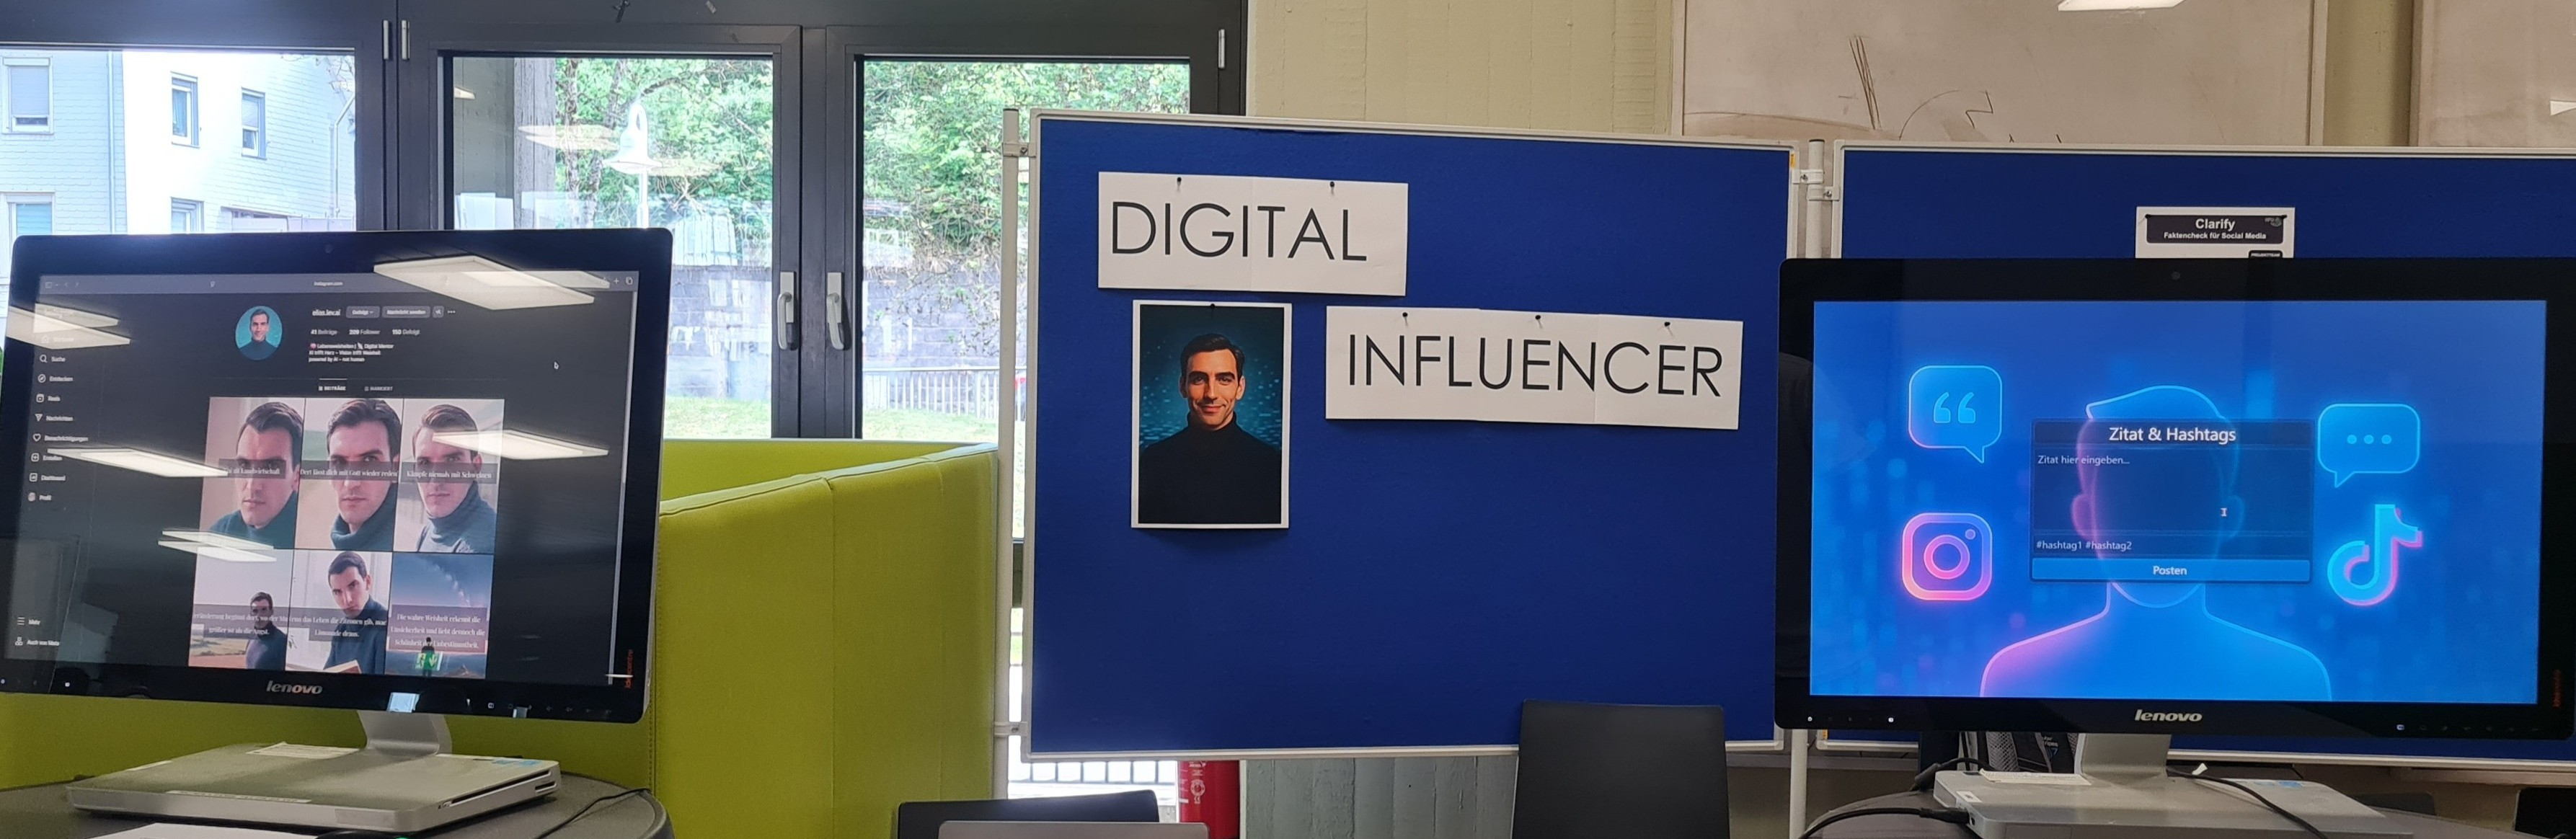
\includegraphics[width=0.98\textwidth]{images/220250704_110638.jpg}
\end{figure}


\subsection{Auszeichnung durch M\&M Software}

Im Rahmen der Veranstaltung vergab die Firma \textbf{M\&M Software} einen mit 500€ dotierten Preis für das beste Informatikprojekt. Unser Team wurde hierbei als \textbf{Gewinner} ausgezeichnet.

In der Begründung hob die Jury hervor:

\begin{itemize}
    \item dass wir zahlreiche technische und organisatorische Hürden (z.\,B. API-Zugänge, DSGVO-Konformität, Toolauswahl) erfolgreich gemeistert haben, die andere Gruppen gar nicht erst betreffen mussten,
    \item dass wir ein vollständig funktionierendes, integriertes System vorweisen konnten,
    \item und dass wir als einzige Gruppe ein interaktives, publikumsfähiges Live-Feature vor Ort bereitstellten, das zuverlässig lief.
\end{itemize}

Die Auszeichnung war für uns ein besonders motivierender Abschluss des Projekts und bestätigte den hohen Anspruch, den wir uns in der Konzeption, Umsetzung und Präsentation gesetzt hatten.

\begin{figure}[h] % [h] = hier einfügen (approx.)
  \centering
  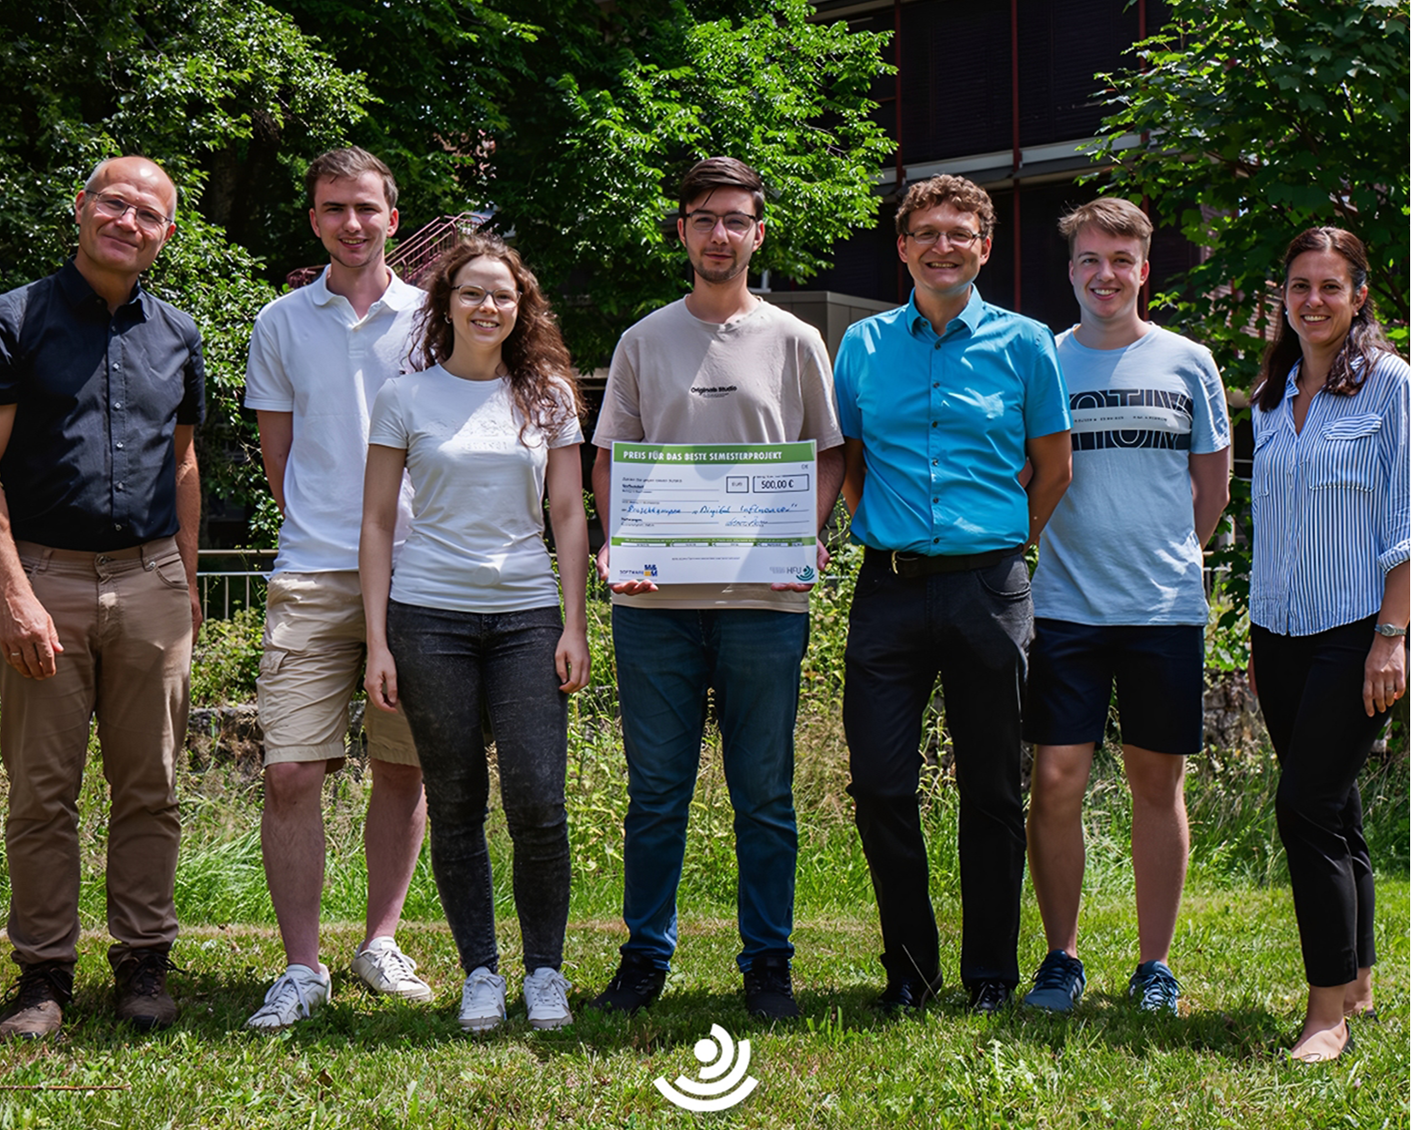
\includegraphics[width=0.8\textwidth]{images/Untitled-1.png}
\end{figure}

\section{Fazit und Zukunftsaussichten}

Das Projekt „Digital Influencer“ verband kreative Ideen mit anspruchsvoller technischer Umsetzung: von der KI-basierten Text- und Bildgenerierung über die vollständig automatisierte Veröffentlichung auf Instagram bis hin zur datenschutzkonformen Interaktion mit der Community. Trotz zahlreicher technischer und organisatorischer Herausforderungen ist es gelungen, ein funktionierendes Gesamtsystem zu entwickeln, das nicht nur in der Theorie überzeugt, sondern auch in der Praxis zuverlässig arbeitet – wie nicht zuletzt die Auszeichnung am Tag der Informatik gezeigt hat.

\subsection{Reflexion}

Rückblickend lässt sich festhalten, dass insbesondere die Integration verschiedener Technologien (z.\,B. lokale LLMs, GitHub Actions, Meta Graph API) zu einem zentralen Erfolgsfaktor wurde. Der modulare Aufbau der Python-Skripte, die Automatisierung wiederkehrender Prozesse sowie die saubere Trennung zwischen generativem Inhalt und Systemlogik machen das System nicht nur funktional, sondern auch gut wartbar und erweiterbar.

Zugleich hat das Projekt auch gezeigt, wie wichtig ein tiefes Verständnis der rechtlichen Rahmenbedingungen – etwa im Bereich Datenschutz oder Plattformrichtlinien – für KI-basierte Social-Media-Systeme ist. Viele ursprünglich angedachte Features (z.\,B. DM-Antworten, dynamische Zielgruppenanpassung) mussten im Sinne der DSGVO gestrichen oder angepasst werden.

\subsection{Mögliche Weiterentwicklungen}

Das aktuelle System bietet eine stabile Grundlage für zahlreiche Erweiterungen, beispielsweise:

\begin{itemize}
    \item \textbf{Videogenerierung integrieren:} Mit zunehmender Verfügbarkeit günstiger oder Open-Source-fähiger Tools könnte ein automatisierter Workflow zur KI-gestützten Reel-Erstellung entstehen – ein Schritt, der die Reichweite auf Instagram nochmals deutlich steigern würde.
    \item \textbf{Feedback-Loop implementieren:} Durch Auswertung der Engagement-Daten (z.\,B. Likes, Saves, Kommentare) könnten in Zukunft Inhalte stärker datenbasiert angepasst werden. Eine Art „Lernmechanismus“ für Themen, Hashtags und Bildsprache.
    \item \textbf{Erweiterung auf andere Plattformen:} Die Grundidee ließe sich auch auf andere Social-Media-Plattformen übertragen (z.\,B. LinkedIn, TikTok) – vorausgesetzt, entsprechende APIs und Nutzungsbedingungen lassen dies zu.
\end{itemize}

\subsection{Lerngewinn für das Team}

Neben den fachlichen Kompetenzen im Bereich KI, API-Nutzung und Automatisierung war das Projekt vor allem auch eine wertvolle Erfahrung in puncto Teamorganisation, Problemlösung unter realen Einschränkungen und zielgruppengerechter Kommunikation.

Dass trotz Limitierungen (z.\,B. kein Business-Status, eingeschränkter API-Zugang, Datenschutzauflagen) ein stimmiges und praxistaugliches Gesamtkonzept entstanden ist, spricht für die Qualität der Planung und Umsetzung. Auch der professionelle Auftritt am Tag der Informatik zeigte: Technische Exzellenz allein reicht nicht – es kommt auf kreative Präsentation und Nutzerorientierung gleichermaßen an.


\section{Arbeitsaufteilung}
In bestimmten Projektabschnitten – wie etwa bei der Marktanalyse, den rechtlichen Grundlagen oder dem Auf- und Abbau des Stands am Tag der Informatik – arbeiteten alle vier Teammitglieder gemeinsam. In anderen Bereichen erfolgte die Umsetzung arbeitsteilig.

Die folgende Übersicht zeigt die jeweiligen Verantwortungsbereiche der einzelnen Mitglieder in Bezug auf Entwicklung und Dokumentation.

\subsubsection*{Marvin}

\begin{itemize}
    \item Entwicklung des automatisierten Posting-Prozesses (\texttt{auto\_post.py}, \texttt{daily\_run.py}, \texttt{weekly\_run.py})
    \item Verwaltung und Einrichtung von GitHub Secrets und Actions
    \item Automatische Zitatgenerierung (\texttt{generate\_content.py})
    \item Gestaltung der Zitatbilder (Textplatzierung auf generierten Motiven)
    \item Entwicklung eines Skripts um automatisch allen Followern ebenfalls zu folgen (\texttt{auto\_refollow.py})
    \item Dokumentation: Technologieauswahl (Python, GitHub, Ollama), Automatisierung (Zitatgenerierung, automatisches Posten, geplante Ausführungen, Archivierung und Rückverfolgbarkeit), Herausforderungen (Erste Versuche mit instagrapi)
\end{itemize}

\subsubsection*{Julia}

\begin{itemize}
    \item Organisation des Zugangs zur offiziellen Meta Graph API (inkl. Token-Erstellung und Verwaltung)
    \item Entwicklung des Systems zur automatischen Kommentarbeantwortung (\texttt{answer\_comments.py}, vorherige Recherche über andere Interaktionen mit Followern)
    \item Programmierung der interaktiven App für den Tag der Informatik (\texttt{manually\_create\_post.py}, Idee hierfür stammt von Marvin)
    \item Followeranalyse (technisch und rechtlich konform bei geringer Followerzahl, \texttt{follower\_analyse.py})
    \item Dokumentation: Layout Überarbeitung, Rechtliche Ausgangslage, Technologieauswahl (Meta Graph API), Automatisierung (Interaktion mit Community), Followeranalyse, Herausforderungen (Datenschutz, Zugang zur Graph API), Tag der Informatik, Fazit und Zukunftsaussichten, Arbeitsaufteilung
\end{itemize}

\subsubsection*{Kevin}

\begin{itemize}
    \item Erstellung der Persona Elias Lev inklusive Steckbrief und Charakter
    \item Prompt-Erstellung und technische Umsetzung der Bildgenerierung (sowohl händisch als auch per API: \texttt{fooocus\_image\_generation\_scripts})
    \item Aufbau einer eigenen Infrastruktur (Organisation und Verwaltung einer Hochschul-VM)
    \item Dokumentation: Deckblatt, Einleitung, Toolrecherche, KI Influencer Persona, Automatisierung (Bildgenerierung), Herausforderungen (Bildgenerierung)
\end{itemize}

\subsubsection*{Bünyamin}

\begin{itemize}
    \item Recherche zu KI-gestützter Videogenerierung
    \item Toolrecherche zu KI-gestützter Bildgenierung (Fooocus)
    \item Dokumentation: Marktanalyse, Toolrecherche, Technologieauswahl (Fooocus), Herausforderungen (Videogenerierung)
\end{itemize}

\subsubsection*{Gemeinsame Leistungen}

\begin{itemize}
    \item Recherche zu bestehenden Tools, rechtlichen Rahmenbedingungen und Plattformvorgaben
    \item Gemeinsame Entwicklung der Projektidee und strategischen Ausrichtung
    \item Marktanalyse, Zielgruppenfestlegung und Positionierung
    \item Aufbau, Abbau und Betreuung des Projektstands am Tag der Informatik
\end{itemize}

\end{document}
